% *****************************************************
%
% IMPLEMENTATION - Describe the work undertaken and the 
% results obtained. Small sections of code can
% be used to aid the understanding of a particular
% point. Discuss testing strategy and show testing 
% details.
%
% *****************************************************
\chapter{Implementation and Testing}
This chapter discusses the tasks that were completed during the implementation phase of this project. It is broken down into the different sections/components of the system and includes the testing strategies that were used to test the completeness and functionality of each feature of the system. To see the full source code, visit the link provided in Appendix \ref{app:product}.
\section{Core chatterbot}
The core of the chatterbot was implemented in Python. It was adapted from two repositories on GitHub at the following links:\\\\
\url{https://github.com/jerryxu178/Chatbot-Eliza}\\
\url{https://github.com/jezhiggins/eliza.py}\\\\
The chatterbot is mainly made up of a dictionary of patterns and corresponding responses, which will be used to match a message from the user to a pattern in the dictionary and respond with a random response from the dictionary. In psychology, the type of language used in this dictionary is known as psychobabble. Figure \ref{fig:psychobabble-example} shows a small snippet of what the dictionary looks like. The dictionary includes a pattern as the key for each item in the dictionary. The `r' at the front of each pattern denotes that the phrase uses regular expressions, so the string is not parsed as a normal string, but is parsed as a regular expression by the in-built regular expressions library. The value associated with each key is a dictionary of responses and most of the responses includes a `{0}' in the string. This will be replaced by the text that falls within the brackets in the pattern associated with the response. For example, given the input ``I need to go meet my mother today", the pattern that will be matched will be ``r`I need (.*)'". If the response is ``Why do you need {0}?", the response displayed to the user will be ``Why do you need to go meet your mother today?". The reason why the response doesn't say ``meet my mother" is because a process to reflect personal pronouns occurs to change the pronoun used in the response. This happens by going through each word in the response and checking if the pronoun is in a pre-defined dictionary of pronouns and if it does replacing it with the corresponding reflected pronoun.

\begin{figure}[h]
	\centering
	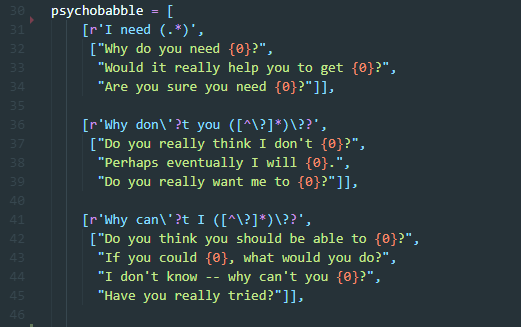
\includegraphics{psychobabble-example}
	\caption{A small snippet of code showing what the psychobabble dictionary looks like.}
	\label{fig:psychobabble-example}
\end{figure}
\section{Long-Term memory mechanism}
% talk about spacy and show snippet of code that does ner 
% also talk about how i get conversation and put it back in conversation
The long-term memory mechanism utilises \gls{ner} and to implement this the spaCy library is used to quickly pass in input to a in-built model. The `en\_core\_web\_md' model is used, which is trained on a web corpus from Wikipedia. Entities are extracted by passing in the input into the model as shown in Figure \ref{fig:ner-extraction}. The entities extracted are added to a JSON object, which includes the entity extracted from the text as the key and the full sentence and the entity type (label) as the values. These entities are passed back to the user interface once the response has been formulated, which can then be added to the database. \\

\begin{figure}[h]
	\centering
	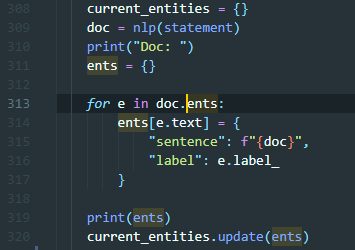
\includegraphics{ner-extraction}
	\caption{Figure showing how entities are extracted from user input}
	\label{fig:ner-extraction}
\end{figure}
\noindent
The following steps take place in the process of interrupting the conversation flow to access the memory:
\begin{enumerate}
	\item The chatterbot core finds a match for the user input from the psychobabble and returns a random response.
	\item The response is then checked to see if the response is appropriate enough to access the memory. It does this by using a regular expression to check for square brackets in the response. As seen in Figure \ref{fig:square-brackets-responses}, some responses contain square brackets, which include some placeholder text for the entity labels accounted for.\\
	\item If there isn't a match for the regular expression, the original response is returned. If there is a match, the match is split into the individual labels so that it is easier to know which entity types can be substituted into the response.
	\item If any entities have just been extracted, the dictionary containing the entities will be checked to see if there are any with the same entity type as one of the placeholders. If there are the placeholder will be replaced by the entity and if the response is not in the recent memory, the response will be returned.
	\item If no entities have been extracted recently, the past entities will be accessed and if the entity has not been talked about recently, the chatterbot will return the following response, where ``[ENTITY]" will be replaced by an actual entity:\\
	\textbf{``Let's change focus. Previously you have talked to me about [ENTITY]. Please tell me more."}
\end{enumerate}
\begin{figure}[h]
	\centering
	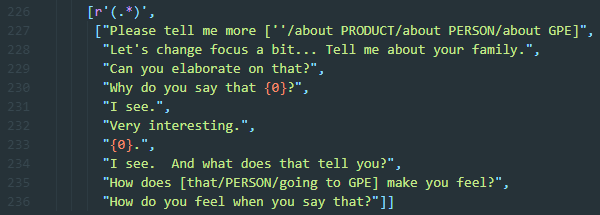
\includegraphics{square-brackets-responses}
	\caption{Figure showing some entities containing placeholder text for some entity labels.}
	\label{fig:square-brackets-responses}
\end{figure}

\section{User Interface}
% talk about how i adapted from GitHub repo and also talk about web sockets
The user interface was adapted from the following GitHub repository:\\\\
\url{https://github.com/keithweaver/eliza}\\\\
It is written in HTML5, CSS3 and JavaScript, using the Bootstrap framework for the front-end. For user authentication, Firebase Authentication service was used and the FirebaseAuth-UI library was used to make it easier to implement the authentication flow and so the front-end of the authentication service did not have to be implemented.\\\\
When the user signed up, a chat node was created first, with a UUID acting as the chat id before the user node was created in the database with the email being the unique id and the chat id of the chat node created being added to the user node to make a reference to the chat the user is associated with. When the user logs in, all the messages, which are stored in the messages sub-collection of the chat node, and entities, which are stored in the users node, are retrieved from the database. The chat messages are then displayed on the screen before the interface connects to a web socket, which emits a message to the chatterbot notifying it to send a greeting. When the user sends a message, the message is displayed and the socket which the chatterbot is connected to, emits the message along with all the entities. When the response is returned, the response is displayed and then sent to the database along with any entities that have been extracted.
\section{Testing}
% talk about how i tested overall system. Console logs, chat logs etc...
To test the authentication flow, messages were printed to the console, to debug where in the flow the program had been executed. This was useful as initially, there were problems with signing up and creating the chat and user node correctly. This testing strategy helped see which functions were being executed and in which order. \\\\
To test the chatterbot, again messages were printed to the console to see the responses, see what matches were being made and also what entities were being extracted. To test the memory mechanism, the different dictionaries that were being used as memory, such as the past entities, current entities and recent responses, were logged to the console to see if the logic that was implemented was correct and if they were being used as expected.\\\\
To test the overall system at the end of the implementation phase, the chatterbot was used as intended and the chat logs were viewed to see if the responses being formulated by the chatterbot were as expected and if the memory mechanism was picking up any topics of conversation in the past. 
\section{Summary}
This chapter gave the reader a detailed insight into the implementation details of this project. It looked at how the core of the chatterbot, long-term memory and user interface were implemented and subsequently pieced together. This chapter also gave the reader information about how the system was tested for completeness and functionality. Where appropriate, snippets of code were given to explain exactly how a certain feature was implemented.\\\\
The next chapter will discuss how the system was evaluated to test how far the system goes in achieving the aims and objectives of this project.